\newsection{Results}{sec:results}

All results in this section were produced on 13 November 2026 on a laptop (Apple Silicon, macOS, Python 3.12.14) against the running Docker Compose stack. The raw outputs are saved in the project under \texttt{report/latex/results/}.

\subsection{Automated Backend Tests}
The backend test suite was run with \texttt{pytest}: \textbf{83 tests passed and 0 failed} in 11.1 seconds. Of these, 68 are unit tests of the business rules and algorithms, and 15 are integration tests that run against real PostgreSQL 16 and Redis 7.

\needspace{7\baselineskip}
\begin{xltabular}{\textwidth}{|p{5.2cm}|>{\centering\arraybackslash}p{1.3cm}|Y|}
\caption{Backend test results by file}\\
\hline
\textbf{Test file} & \textbf{Tests} & \textbf{What it checks} \\ \hline
unit/test\_domain\_invariants & 10 & Entity validation and state-machine transitions \\ \hline
unit/test\_hardening & 10 & File-type sniffing, size, pixel and page limits \\ \hline
unit/test\_task\_maths & 9 & Priority score ranges, alert times, completion rate \\ \hline
unit/test\_ocr\_maths & 8 & Length-weighted confidence, time grammar, deskew \\ \hline
unit/test\_parsers & 6 & Excel merged cells, CSV, PDF tables, cell tokens \\ \hline
unit/test\_initials\_matching & 4 & Exact, alias, fuzzy and ambiguous initials \\ \hline
unit/test\_reminder\_maths & 4 & Fire time, idempotency key, back-off, quiet hours \\ \hline
7 other unit files & 17 & Clash detection, free slots, recurrence, ICS, clock, policy, bulk import \\ \hline
8 integration files & 15 & Log-in flow, timetable, circular, calendar, task and reminder pipelines, rate limiter, repositories \\ \hline
\textbf{Total} & \textbf{83} & \textbf{All passed} \\ \hline
\end{xltabular}

\subsection{End-to-End Browser Tests}
Four user journeys were run in a real Chromium browser with Playwright against the running frontend and API: \textbf{4 passed} in 12.9 seconds.

\needspace{7\baselineskip}
\begin{xltabular}{\textwidth}{|>{\centering\arraybackslash}p{1.2cm}|Y|>{\centering\arraybackslash}p{1.4cm}|>{\centering\arraybackslash}p{1.4cm}|}
\caption{End-to-end test results}\\
\hline
\textbf{No.} & \textbf{Journey verified in the browser} & \textbf{Result} & \textbf{Time} \\ \hline
1 & HOD uploads \texttt{standard\_timetable.xlsx} and confirms; faculty KKS sees the classes on the calendar & Pass & 3.7 s \\ \hline
2 & Faculty uploads a circular; HOD reviews and confirms; attendees see the meeting & Pass & 5.0 s \\ \hline
3 & A scheduled meeting produces a notification record marked SENT & Pass & 0.6 s \\ \hline
4 & HOD assigns a template task; faculty completes it; pending alerts are resolved & Pass & 2.2 s \\ \hline
\end{xltabular}

\subsection{Algorithm Outputs on Worked Examples}
The values below were computed by calling the project's own functions with the time fixed at 04:30 UTC on 13 November 2026 (script \texttt{results/worked\_examples.py}).

\head{Task Priority Score}
\begin{table}[H]
\centering
\begin{tabular}{|p{4.8cm}|>{\centering\arraybackslash}p{2.2cm}|>{\centering\arraybackslash}p{3.2cm}|>{\centering\arraybackslash}p{2.4cm}|}
\hline
\textbf{Task} & \textbf{Importance} & \textbf{Hours to deadline} & \textbf{Priority $P$} \\ \hline
IA marks upload & 5 & 6 & 0.9295 \\ \hline
CO--PO mapping & 4 & 48 & 0.5207 \\ \hline
Lab manual update & 2 & 240 & 0.1040 \\ \hline
Course file submission & 3 & $-36$ (overdue) & 1.2143 \\ \hline
\end{tabular}
\caption{Priority scores of four sample tasks}
\end{table}
The overdue task ranks first, then the urgent high-importance task. For example, IA marks upload scores $0.4 \times 4/4 + 0.6 \times e^{-6/48} = 0.4 + 0.5295 = 0.9295$.

\head{Initials Similarity}
\begin{table}[H]
\centering
\begin{tabular}{|p{2.6cm}|p{2.6cm}|>{\centering\arraybackslash}p{2.4cm}|p{5.2cm}|}
\hline
\textbf{Token} & \textbf{Candidate} & \textbf{Similarity} & \textbf{Decision} \\ \hline
KKS & KKS & 1.000 & Match (exact) \\ \hline
PARKAVI & PARKAVY & 0.857 & Fuzzy match if margin $\ge 0.10$ \\ \hline
KKS & KSS & 0.667 & Rejected (below 0.85) \\ \hline
RNS & KKS & 0.333 & Rejected \\ \hline
\end{tabular}
\caption{Normalised Levenshtein similarity examples}
\end{table}

\head{Other Worked Examples}
\begin{itemize}
  \item \textbf{Quiet hours:} a 10:00 IST class on 14 November with a 12-hour reminder would fire at 22:00 IST, inside a 22:00--07:00 quiet window. The planner moved it to 07:00 IST (01:30 UTC), still before the class.
  \item \textbf{Task alerts:} a task due in 5 days produced alerts exactly 72 hours, 24 hours and 2 hours before the deadline.
  \item \textbf{OCR confidence:} the words ``Meeting on 18/11/2026 at 2:30 PM'' with confidences 96, 91, 72, 88, 65 and 90 give a length-weighted confidence of $2190/27 = 81.11$, above the gate of 70.
\end{itemize}

\subsection{Clash Detection Performance}
Random 50, 60 or 120-minute events were placed on a 15-minute grid over 30 days (fixed random seed 20261113). The sweep-line detector and the brute-force pairwise check returned identical clash sets at every size.

\begin{table}[H]
\centering
\begin{tabular}{|>{\centering\arraybackslash}p{2.2cm}|>{\centering\arraybackslash}p{2.4cm}|>{\centering\arraybackslash}p{2.6cm}|>{\centering\arraybackslash}p{2.6cm}|>{\centering\arraybackslash}p{2.2cm}|}
\hline
\textbf{Events $n$} & \textbf{Clash pairs} & \textbf{Sweep line (ms)} & \textbf{Pairwise (ms)} & \textbf{Same result} \\ \hline
500 & 444 & 0.14 & 4.53 & Yes \\ \hline
1,000 & 1,667 & 0.31 & 25.78 & Yes \\ \hline
2,000 & 6,697 & 0.91 & 74.34 & Yes \\ \hline
4,000 & 26,822 & 2.47 & 299.06 & Yes \\ \hline
\end{tabular}
\caption{Sweep-line versus brute-force clash detection (one run per size)}
\end{table}

\begin{figure}[!htbp]
\centering
\begin{tikzpicture}
  \begin{scope}[x=0.0028cm, y=0.022cm]
    \draw[semithick, -{Stealth[length=2mm]}] (0,0) -- (4300,0) node[below left, font=\scriptsize] {events $n$};
    \draw[semithick, -{Stealth[length=2mm]}] (0,0) -- (0,330) node[above, font=\scriptsize] {time (ms)};
    \foreach \x in {1000,2000,3000,4000} \draw (\x,0) -- (\x,-5) node[below, font=\tiny] {\x};
    \foreach \y in {100,200,300} \draw (0,\y) -- (-60,\y) node[left, font=\tiny] {\y};
    \draw[semithick] (500,4.53) -- (1000,25.78) -- (2000,74.34) -- (4000,299.06);
    \foreach \p in {(500,4.53),(1000,25.78),(2000,74.34),(4000,299.06)} \fill \p circle (1.4pt);
    \draw[semithick, dashed] (500,0.14) -- (1000,0.31) -- (2000,0.91) -- (4000,2.47);
    \foreach \p in {(500,0.14),(1000,0.31),(2000,0.91),(4000,2.47)} \draw[fill=white] \p circle (1.4pt);
    \node[font=\scriptsize, anchor=west] at (3000,240) {pairwise $O(n^2)$};
    \node[font=\scriptsize, anchor=west] at (3000,25) {sweep line $O(n \log n + k)$};
  \end{scope}
\end{tikzpicture}
\caption{Clash detection time against the number of events}
\end{figure}

\subsection{Database Benchmark (Recorded Earlier)}
During the hardening stage on 28 October 2026, a benchmark script loaded 120 faculty, 5,000 tasks and two terms. A one-week calendar query took 0.60 ms at the 95th percentile, and claiming 1,000 due notifications took 1.2 ms. This benchmark was not rerun for this report.

\subsection{Application Screens}
The screens below were captured by an automated Playwright script from the running application, logged in with the seeded test accounts.

\begin{figure}[!htbp]
  \centering
  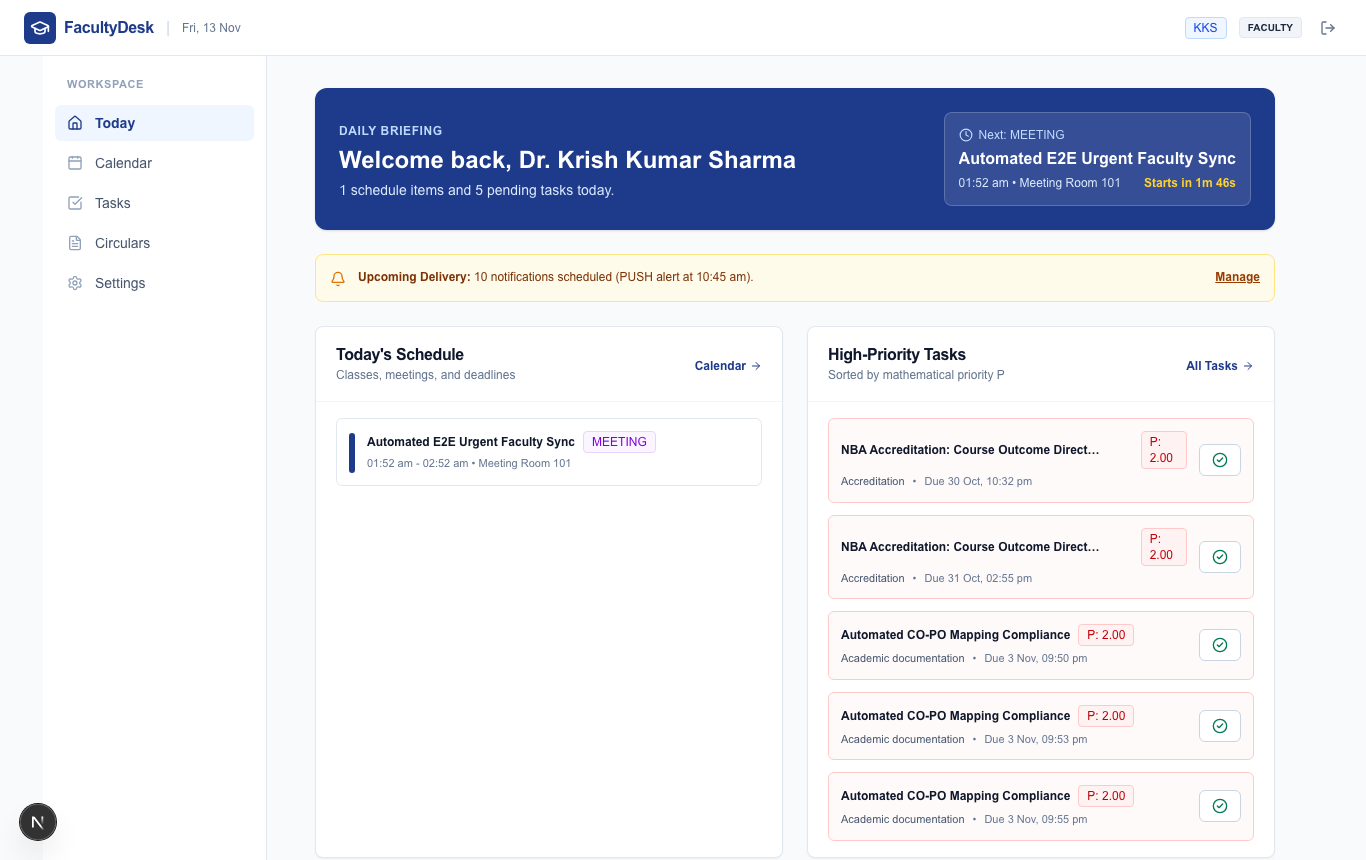
\includegraphics[width=0.92\textwidth]{figures/screens/faculty-today.png}
  \caption{Faculty ``Today'' screen: next meeting countdown, today's schedule and high-priority tasks}
\end{figure}
\begin{figure}[!htbp]
  \centering
  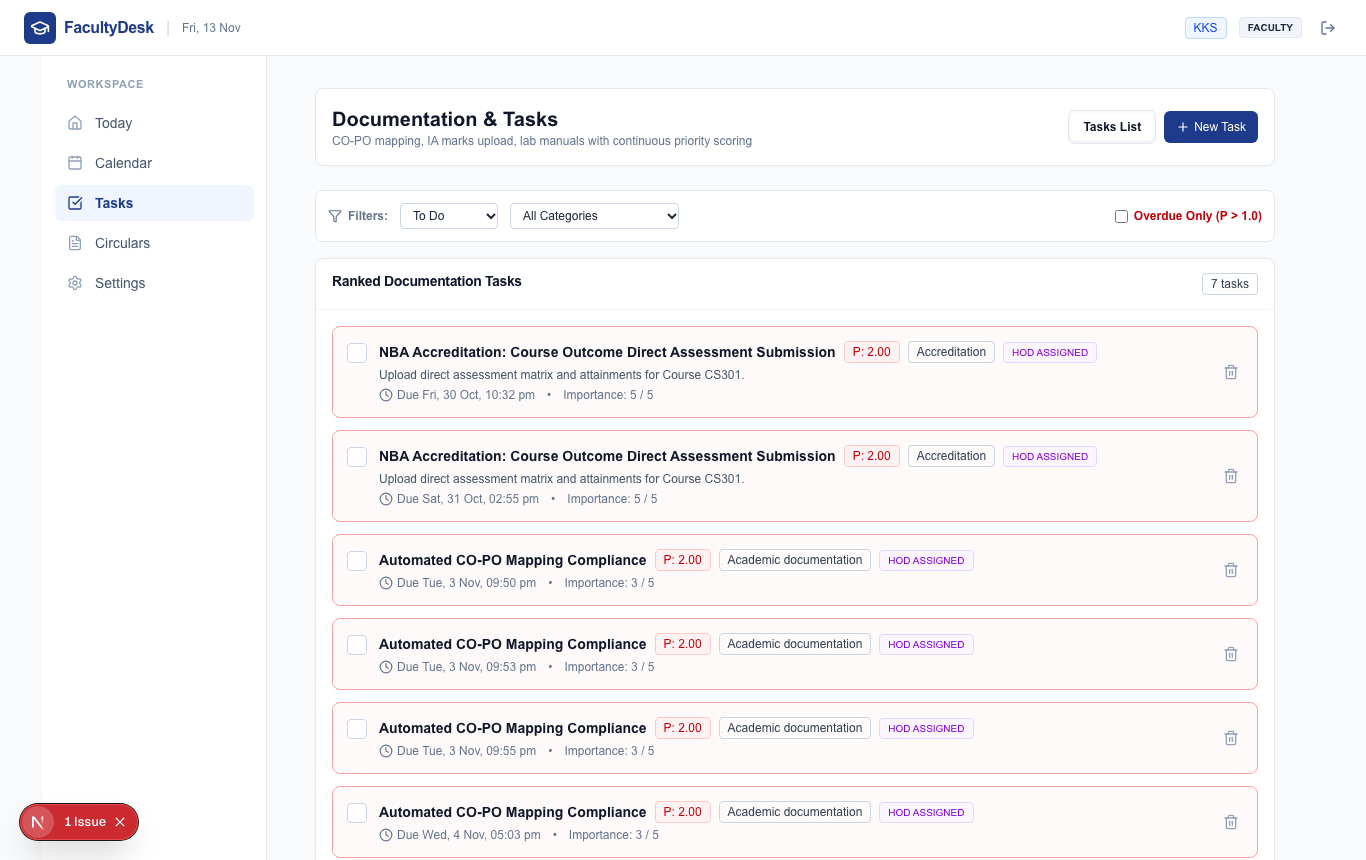
\includegraphics[width=0.92\textwidth]{figures/screens/faculty-tasks.png}
  \caption{Documentation tasks ranked by priority score $P$ (overdue tasks have $P > 1$)}
\end{figure}
\begin{figure}[!htbp]
  \centering
  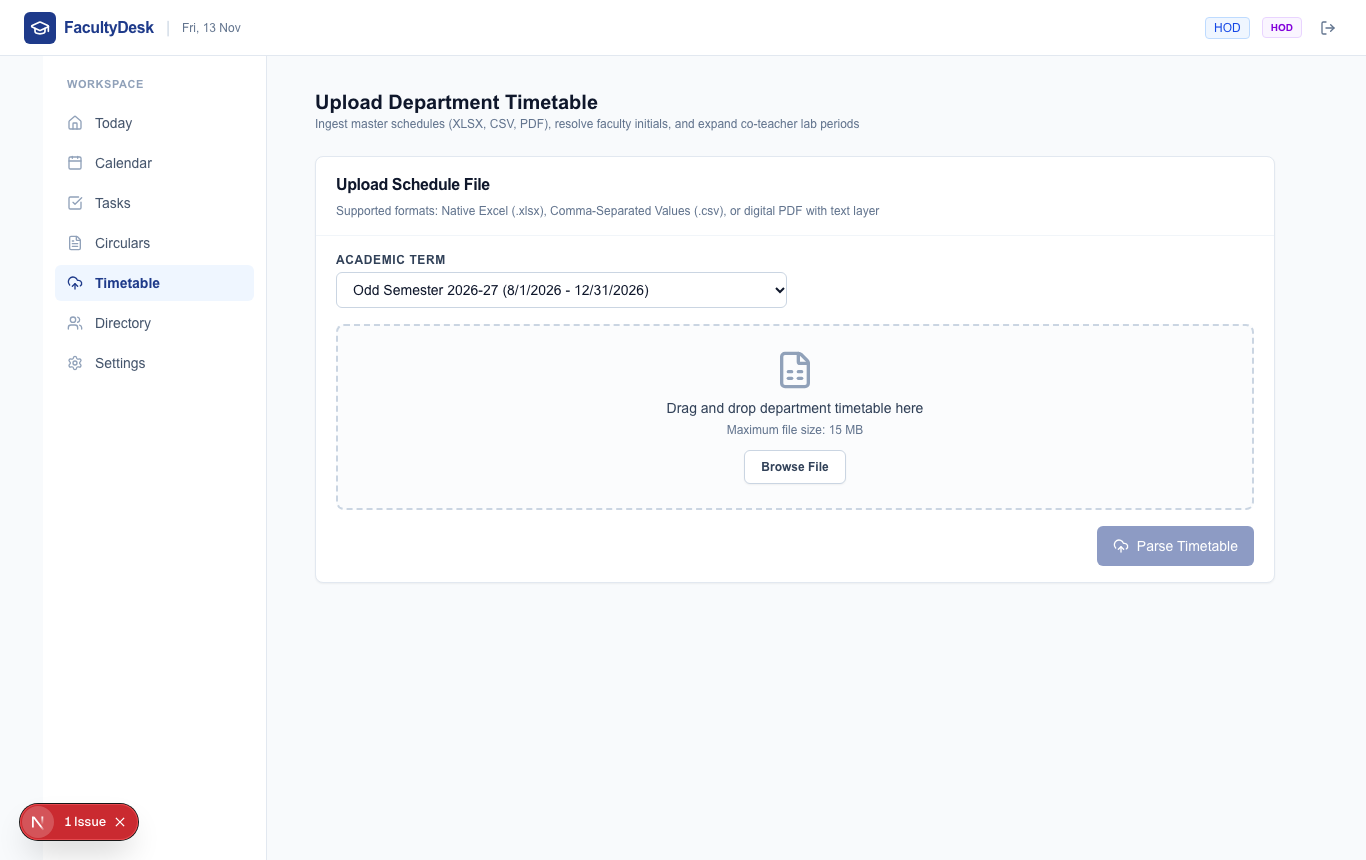
\includegraphics[width=0.92\textwidth]{figures/screens/hod-timetables.png}
  \caption{HOD timetable upload screen}
\end{figure}
\begin{figure}[!htbp]
  \centering
  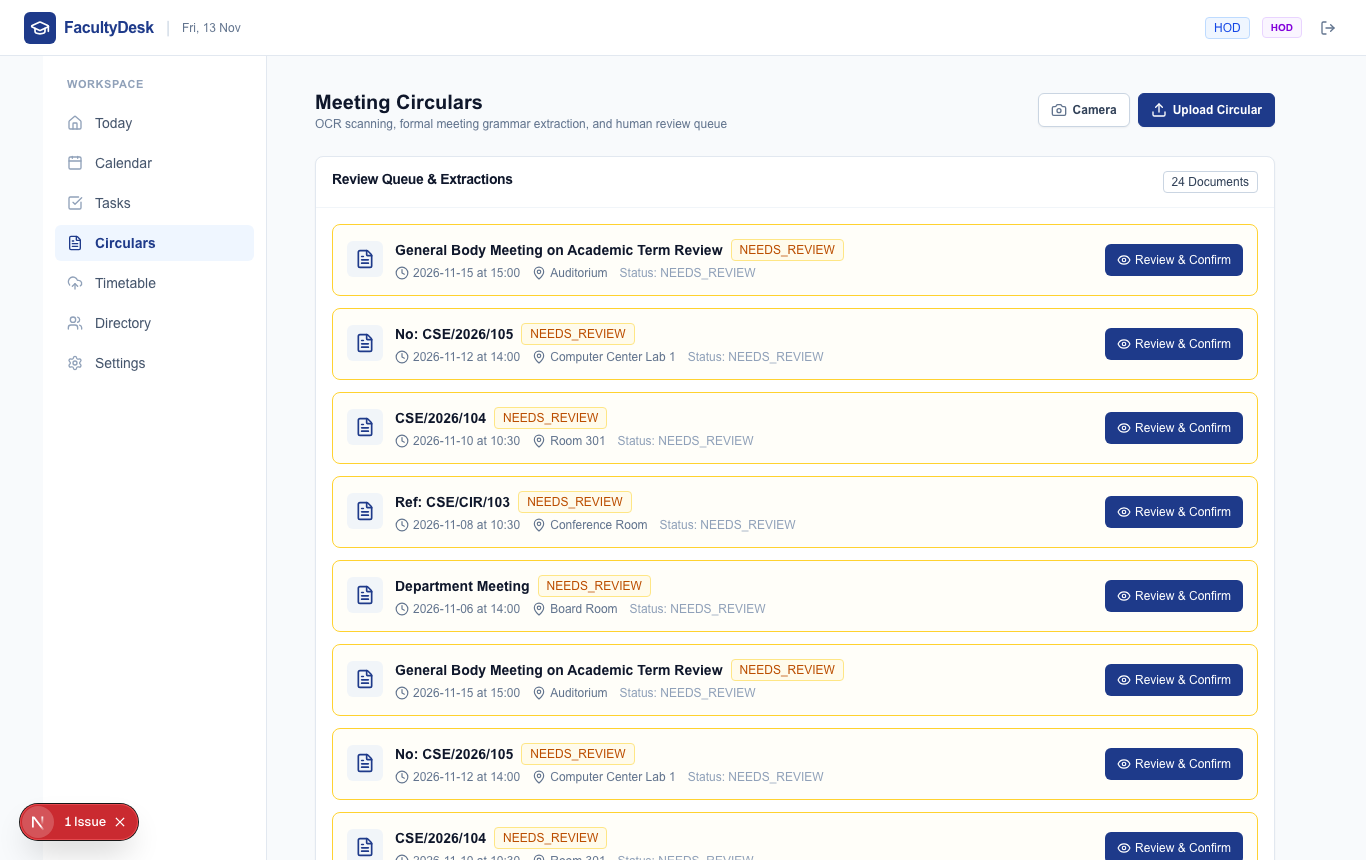
\includegraphics[width=0.92\textwidth]{figures/screens/hod-circulars.png}
  \caption{HOD circular review queue with OCR-extracted date, time and venue}
\end{figure}
\begin{figure}[!htbp]
  \centering
  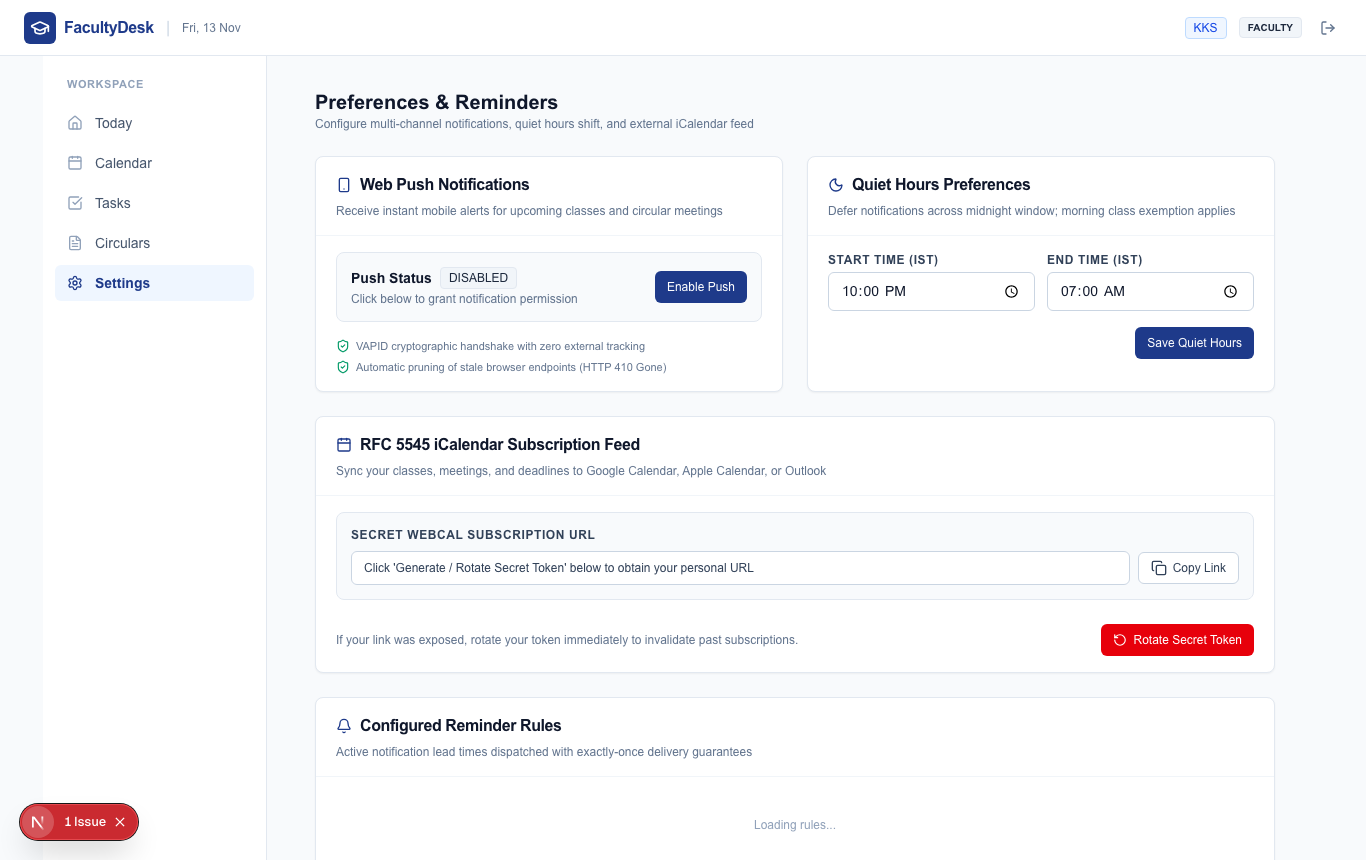
\includegraphics[width=0.92\textwidth]{figures/screens/faculty-settings.png}
  \caption{Reminder settings: web push, quiet hours and private ICS feed}
\end{figure}
